% =====================================================================
%  CITS4012 Group Project -- PIQA
%
%  TO BUILD ON OVERLEAF WITH THE REAL ACL TEMPLATE:
%    1. New Project -> Templates -> search "ACL" -> create.
%    2. Upload every file in this folder into it.
%    3. In this file, replace   \usepackage{aclfallback}
%                      with     \usepackage[final]{acl}
%       and delete aclfallback.sty. Nothing else changes.
%
%  aclfallback.sty reproduces the ACL geometry (letter, 1in margins,
%  two columns, 0.2in gutter, 10pt Times) so the file also compiles
%  as-is for checking the page count.
%
%  compact.sty holds every layout knob in one place -- float spacing,
%  caption size, display-maths skips. Turn those to trade whitespace
%  for pages without touching a word of the text.
% =====================================================================
\documentclass[11pt]{article}
\usepackage[preprint]{acl}           % official ACL style file (preprint shows page numbers)
\usepackage{times}
\usepackage[T1]{fontenc}
\usepackage[utf8]{inputenc}
\usepackage{microtype}
\usepackage{graphicx}
\usepackage{amsmath,amssymb}
\usepackage{booktabs}
\usepackage{colortbl}             % \rowcolor for the "Ours" rows in Table 3
\definecolor{ourrow}{RGB}{226,238,248}
\usepackage{compact}

\title{Attention over Near-Duplicate Candidates on PIQA:\\Separating Noise From Signal}
\author{Group 15}
\date{}

\begin{document}
\maketitle

\begin{abstract}
  The two candidate solutions of a PIQA instance are near-duplicates,
  overlapping by $0.653$ on average, so we condition attention on the goal and
  add a parameter-free residual aligning each candidate against the other.
  Against a pooled seed-noise threshold of $0.0099$, no attention
  configuration separates from a no-attention backbone. The baselines locate
  the gain elsewhere: a frozen pretrained encoder scores below our model, the
  same checkpoint fine-tuned $6.1$ points above it, and zero-shot Qwen2.5-3B
  $18.0$ points above. At this data scale pretraining, not architecture, moves
  the result.
\end{abstract}

\section{Introduction}
\label{sec:intro}

A PIQA instance gives a short physical goal and two candidate solutions, of
which exactly one is correct \citep{bisk2020piqa}. The benchmark tests whether
a system understands the physical consequences of an action, a capability
required for grounded instruction following and embodied planning. Its
difficulty comes from the data: the candidates are near-duplicates,
overlapping by $0.653$ on average, so the evidence separating them sits in a
few disputed positions.

We set out to test whether attention designed for that structure can recover
the signal, and to measure any gain against the noise the training procedure
generates on its own. One bidirectional LSTM encodes all three inputs; a
goal-conditioned
bilinear attention \citep{luong2015attention} lets the goal decide which words
of a candidate matter; and a parameter-free cross-attention residual
\citep{chen2017esim} passes the scorer only what one candidate cannot account
for in the other. Each component switches off
independently, and differences are judged against a $0.0099$ threshold pooled
from the seed noise of sixteen configurations.

Nothing inside the architecture moves the result: the best attention
configuration gains $0.0039$ over plain mean pooling, and the weights show why
--- those that perform best are the flattest, which is mean pooling under
another name. What moves the result is pretraining scale.

\section{Methodology}
\label{sec:method}

\subsection{Task formulation and notation}
\label{sec:task}

An instance is a goal $g$, candidates $s_1,s_2$ of which exactly one is
correct, and a label $y \in \{1,2\}$. We score rather than classify a
concatenated input: $f$ takes the goal, the candidate scored and its
competitor, returning an unnormalised real number:
\begin{equation}
\hat{y} \;=\; \operatorname*{arg\,max}_{k \in \{1,2\}} \; f(g,s_k,s_{3-k}).
\label{eq:argmax}
\end{equation}
A softmax over the two feeds the cross-entropy loss; because both pass
through the same $f$, their scores share a scale and the prediction is
independent of their order.

\subsection{The characteristics of PIQA that drive the design}
\label{sec:hard}

Figure~\ref{fig:task}(a), a representative training instance, shows two
candidates differing by a single word, and that word decides the answer.

\begin{figure}[tb]
  \centering
  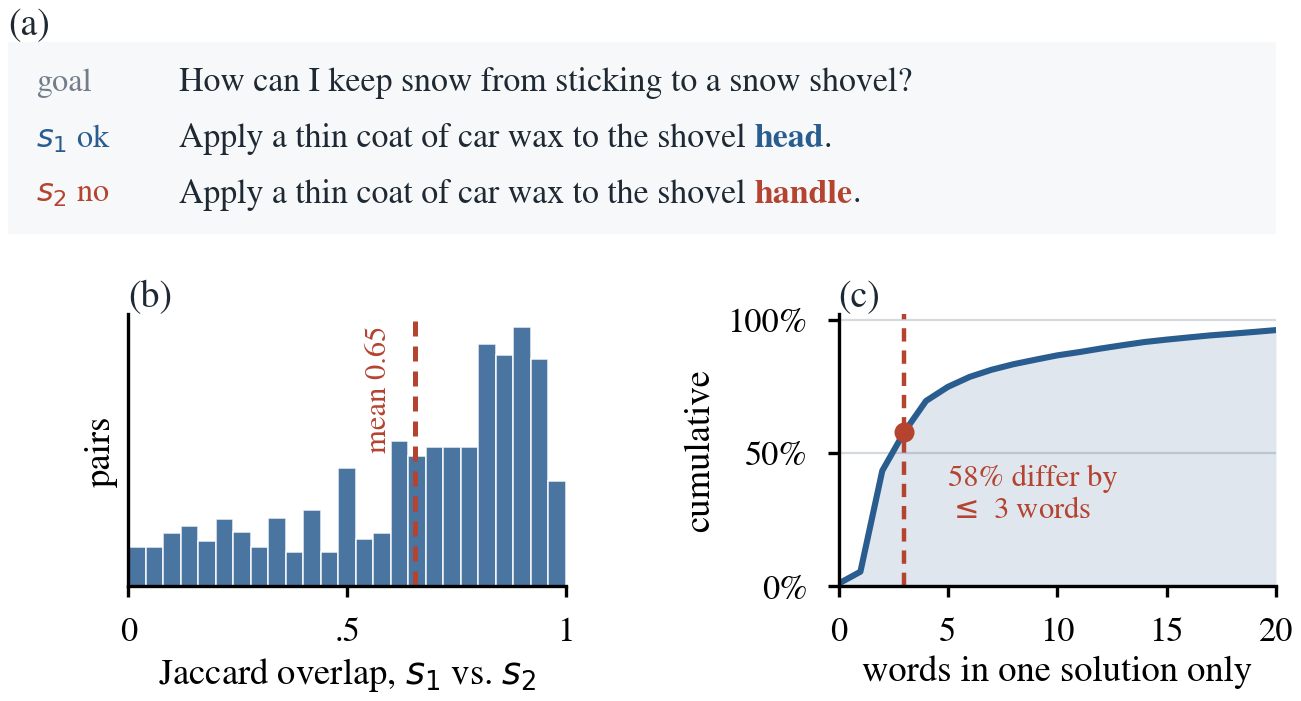
\includegraphics[width=0.82\columnwidth]{fig1_task.png}
  \caption{(a) A training instance whose candidates differ by one word.
  (b) Jaccard overlap of $s_1$ and $s_2$. (c) Words in only one candidate.}
  \label{fig:task}
\end{figure}


That instance is typical. Measuring overlap with the Jaccard index over
distinct preprocessed tokens, $J = |W(s_1) \cap W(s_2)| / |W(s_1) \cup
W(s_2)|$, it exceeds $0.8$ in $37.5\%$ of training pairs, and $57.9\%$ differ
by three words or fewer (Figure~\ref{fig:task}b,~c). The candidates are
near-duplicates: whatever separates them sits in a handful of positions.
Three decisions follow.

\begin{description}
  \item[D1] \textit{One encoder and scorer are shared across all three
  inputs,} so any difference reported between the candidates originates in
  the text.
  \item[D2] \textit{The goal determines which words of a candidate matter,}
  so it constructs the attention query rather than being concatenated
  alongside the candidate.
  \item[D3] \textit{The candidates attend to each other.} The discriminative
  signal lies where they disagree, so the scorer receives that residual
  directly. Near duplication is exactly the condition under which such a
  residual carries most of the signal, and D3 is designed for it.
\end{description}

\subsection{Shared encoder}
\label{sec:encoder}

Tokens pass through an embedding matrix $E$ of size $V$ by $d$, trained from
scratch. One bidirectional LSTM \citep{hochreiter1997lstm} encodes all three
inputs, giving states of size $L_g \times 2H$ and $L_s \times 2H$ with
$L_g = 20$, $L_s = 60$, $d = 100$, $H = 100$. Sharing the encoder implements
D1 and extends the Siamese arrangement of \citet{mueller2016siamese} from two
inputs to three; wherever a sequence is reduced to one vector we average over
non-padding positions.

Three alternatives were considered. A vanilla RNN was rejected because
candidates run to 60 tokens and a simple cell loses gradient information over
that span. A GRU reaches $0.5922 \pm 0.0060$ against $0.6003 \pm 0.0032$,
inside the noise floor, so the cell type is not where the improvement lies. A
Transformer was set aside on data scale: the original saw 4.5M sentence pairs
\citep{vaswani2017attention}, three orders of magnitude above our
$13{,}696$.

\subsection{Attention over the candidate and over the goal}
\label{sec:attn}

All three share one form: a query $\mathbf{q}$ scores every position of a
sequence $H$, padding is suppressed before the softmax, and the weights pool
it into one vector:
\begin{equation}
\boldsymbol{\alpha} = \mathrm{softmax}\!\left(\frac{H\mathbf{q}}{T}\right),
\qquad
\mathbf{c} = \sum_i \alpha_i \mathbf{h}_i .
\label{eq:attn}
\end{equation}
The temperature $T$ controls concentration (Section~\ref{sec:refine}). What
distinguishes the three is where the query comes from.

\paragraph{A1, goal-conditioned attention}
The query comes from the goal by a learned bilinear projection
$\mathbf{q} = Wg$. This is the general scoring function of
\citet{luong2015attention} applied between two sequences rather than within a
decoder, implementing D2; we prefer it to a plain dot product because goal
and candidate play different roles --- what is asked against what is proposed
--- and $W$ learns the mapping.

\paragraph{A2, self-attention over the goal}
Rather than averaging the goal's words, we learn a single query vector $q_g$
with $200$ parameters and apply Equation~\ref{eq:attn} to the goal, following
the word-level attention of \citet{yang2016hierarchical}.

\subsubsection{Refinements to goal-conditioned solution attention}
\label{sec:refine}

We refine A1 in three ways, leaving A2 unchanged and masking invalid positions
throughout. Each solution token attends to the non-padding goal tokens in a
low-rank space ($r = 64$) through a gated residual with $\beta$ initialised to
zero; the states are pooled under a learned temperature $T$ initialised to
$\sqrt{D}$; and the attended context is mixed with $\bar{h}_k$, the masked
mean of the original states, by a gate $\lambda = \sigma(\gamma)$ initialised
to $0.5$:
\begin{align}
A_k &= \mathrm{softmax}_j\!\left(
   \tfrac{1}{\sqrt{r}}\left(H^{k}W_{Q}\right)\left(H^{g}W_{K}\right)^{\!\top}
   \!+ M^{g}\right), \nonumber\\
\widetilde{H}^{k} &= H^{k} + \tanh(\beta)\,A_k\!\left(H^{g}W_{V}\right)W_{O},
   \nonumber\\
\boldsymbol{\alpha}_k &= \mathrm{softmax}_i\!\left(
   \tfrac{\widetilde{H}^{k}\mathbf{q} + M^{k}}{T}\right), \nonumber\\
c_k &= \lambda\,\boldsymbol{\alpha}_k^{\!\top}\widetilde{H}^{k}
       + (1-\lambda)\,\bar{h}_k .
\label{eq:refine}
\end{align}
The residual has no effect at initialisation, and only A1 receives enhanced
states. Adapting scaled dot-product attention \citep{vaswani2017attention}
this way costs $51{,}203$ parameters: four bias-free projections plus three
scalars.

\subsection{Cross-attention between the candidates}
\label{sec:cross}

A3 implements D3 by aligning each token of one candidate with every
non-padding token of the other \citep{chen2017esim}, keeping the signed
residual $r^{k}_{i} = h^{k}_{i} - \sum_j \beta^{k}_{ij} h^{3-k}_{j}$ between a
token and what the competing candidate explains of it:
\begin{equation}
d_k = \big[\,\mathrm{maskedMean}_i(r^{k}_{i}); \;
            \mathrm{maskedMax}_i(r^{k}_{i})\,\big],
\label{eq:residual}
\end{equation}
with $d_k \in \mathbb{R}^{4H}$ and $\beta^{k}_{ij} =
\mathrm{softmax}_j\big((h^{k}_{i})^{\!\top} h^{3-k}_{j}\big)$ unscaled over
the original BiLSTM states, so A3 stays independent of A1. The mean captures evidence spread across the candidate and the max preserves
strong local differences; neither adds parameters, though the extra $2H$
vector widens the scorer input to $12H$. Unlike ESIM, our candidates have
symmetric roles, so we pool the residual directly.

\subsection{Interaction features and scoring}
\label{sec:scoring}

The goal, attended candidate summary and alignment residual combine through
the interaction features of \citet{conneau2017infersent}:
\begin{equation}
u_k = \big[\, g; \; c_k; \; g \odot c_k; \; |g - c_k|; \; d_k \,\big]
      \in \mathbb{R}^{12H}.
\label{eq:u}
\end{equation}
The product and absolute difference give the scorer an explicit measure of
agreement and disagreement, and a two-layer feed-forward network with dropout
maps $u_k$ to a scalar. Figure~\ref{fig:arch} shows the complete model:
$1{,}522{,}204$ parameters, $75.5\%$ in the embedding matrix, so close to
three quarters of what it must learn is the word representations themselves.

\begin{figure*}[tb]
  \centering
  \includegraphics[width=0.70\textwidth]{fig2_architecture.pdf}
  \caption{Model architecture. One embedding matrix and one bidirectional
  LSTM encode all three inputs; one scorer runs on each candidate in turn.}
  \label{fig:arch}
\end{figure*}

\section{Experimental Setup}
\label{sec:setup}

\subsection{Dataset and preprocessing}
\label{sec:data}

PIQA provides $16{,}113$ labelled training and $1{,}838$ test instances with
no official validation split, and neither favours one answer position
(Table~\ref{tab:data}).

\begin{table}[tb]
  \centering\small
  \begin{tabular}{@{}lrr@{}}
    \toprule
     & \textbf{train} & \textbf{test}\\
    \midrule
    Instances & $16{,}113$ & $1{,}838$\\
    Proportion with $y = 2$ & $0.500$ & $0.505$\\
    Goal words, mean / p95 & $7.1$ / $13$ & n/m\\
    Candidate words, mean / p95 & $19.6$ / $54$ & n/m\\
    Jaccard overlap, mean & $0.653$ & n/m\\
    Candidates differing by $\leq 3$ words & $57.9\%$ & n/m\\
    Vocabulary, count $\geq 2$ & $11{,}488$ & ---\\
    \bottomrule
  \end{tabular}
  \caption{Dataset statistics. Candidate length is the longer of the two;
  n/m was deliberately not measured.}
  \label{tab:data}
\end{table}

\paragraph{Splits}
We partition the training set $85/15$ stratified on the label, giving
$13{,}696$ training and $2{,}417$ validation instances. Every design decision
and ablation was made on that split; the test set was used once, for
Table~\ref{tab:overall}, with only its size and label balance inspected
beforehand.

\paragraph{Preprocessing}
Text is lower-cased and split on whitespace after punctuation is removed. The
vocabulary comes from the training split alone, holds $11{,}488$ types at a
minimum count of two, and maps unseen words to an unknown index. Sequences are
padded or truncated to $L_g = 20$ and $L_s = 60$, both above the 95th
percentile, so truncation touches $0.2\%$ of goals and $3.5\%$ of
candidates.

\subsection{Training procedure}
\label{sec:training}

Models train with Adam \citep{kingma2015adam} at batch size $32$ under
cross-entropy loss, with dropout on the scorer input; its per-parameter step
matters because the dominant component is an embedding matrix whose rows see
a gradient only in batches holding their word.

\paragraph{Epoch budget}
Every configuration trains for a fixed $15$ epochs and we keep the epoch of
highest validation accuracy; over ten seeds run to $25$ the mean curve
flattens by the fifth, and extending the budget is worth $0.0019$.

\paragraph{Reproducibility}
We seed Python, NumPy and PyTorch every run, set \texttt{cudnn.deterministic}
and disable \texttt{cudnn.benchmark}. Before these controls, repeated runs of
one seed drifted by up to $0.015$, larger than several effects we report;
with them a configuration re-run days later reproduced its three accuracies
exactly. One Tesla T4, torch 2.11.0+cu130.

\paragraph{Noise floor}
A standard deviation from three seeds is unreliable: across sixteen
configurations these estimates span $0.0002$ to $0.0083$, a range we read as
sampling variability. Pooling them gives $0.0049$, so we treat configurations
whose means differ by less than $0.0099$ as indistinguishable, and test larger
differences with Welch's $t$-test.

\subsection{Hyperparameter selection}
\label{sec:hparams}

Hyperparameters were selected one at a time around a fixed reference
configuration, on the validation split with attention disabled
(Figure~\ref{fig:hp}).

\begin{figure*}[tb]
  \centering
  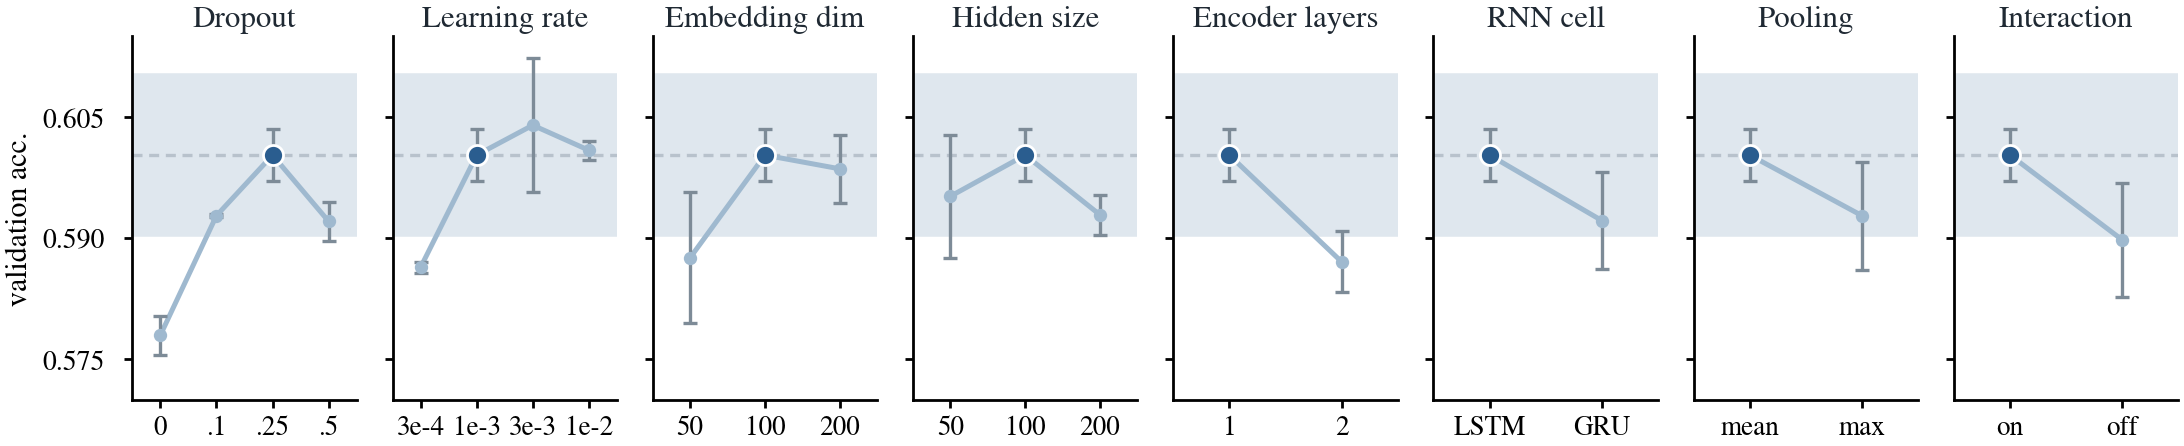
\includegraphics[width=0.99\textwidth]{fig4_hyperparams.png}
  \caption{Validation accuracy for every hyperparameter value tested, three
  seeds per point. Shaded band is the $\pm 2\sigma$ seed noise; the dark
  marker is the value adopted.}
  \label{fig:hp}
\end{figure*}


The adopted configuration is dropout $0.25$, learning rate $0.001$, embedding
width $100$, hidden size $100$, one encoder layer, an LSTM cell, mean pooling,
interaction features on, batch size $32$ and $15$ epochs. Only three settings
fall outside the noise band: removing dropout costs $0.0223$, a second encoder
layer $0.0133$, and removing the interaction features $0.0105$. The other
eight we took the simpler setting --- learning rate $0.003$ scored $0.0037$
above $0.001$ but with a seed spread two and a half times wider.

\subsection{Baseline models}
\label{sec:baselines}

We evaluate against a lexical floor and four baselines spanning different
adaptation strategies: B1 a bag-of-embeddings model trained from scratch, B2a
and B2b the same DistilRoBERTa checkpoint frozen and fine-tuned, and B3
zero-shot Qwen2.5-3B \citep{qwen2024} --- separating what a pretrained
representation contains from what adapting it provides. All use the same split
and seeds; every number is our own (Figure~\ref{fig:base}).

\begin{figure}[tb]
  \centering
  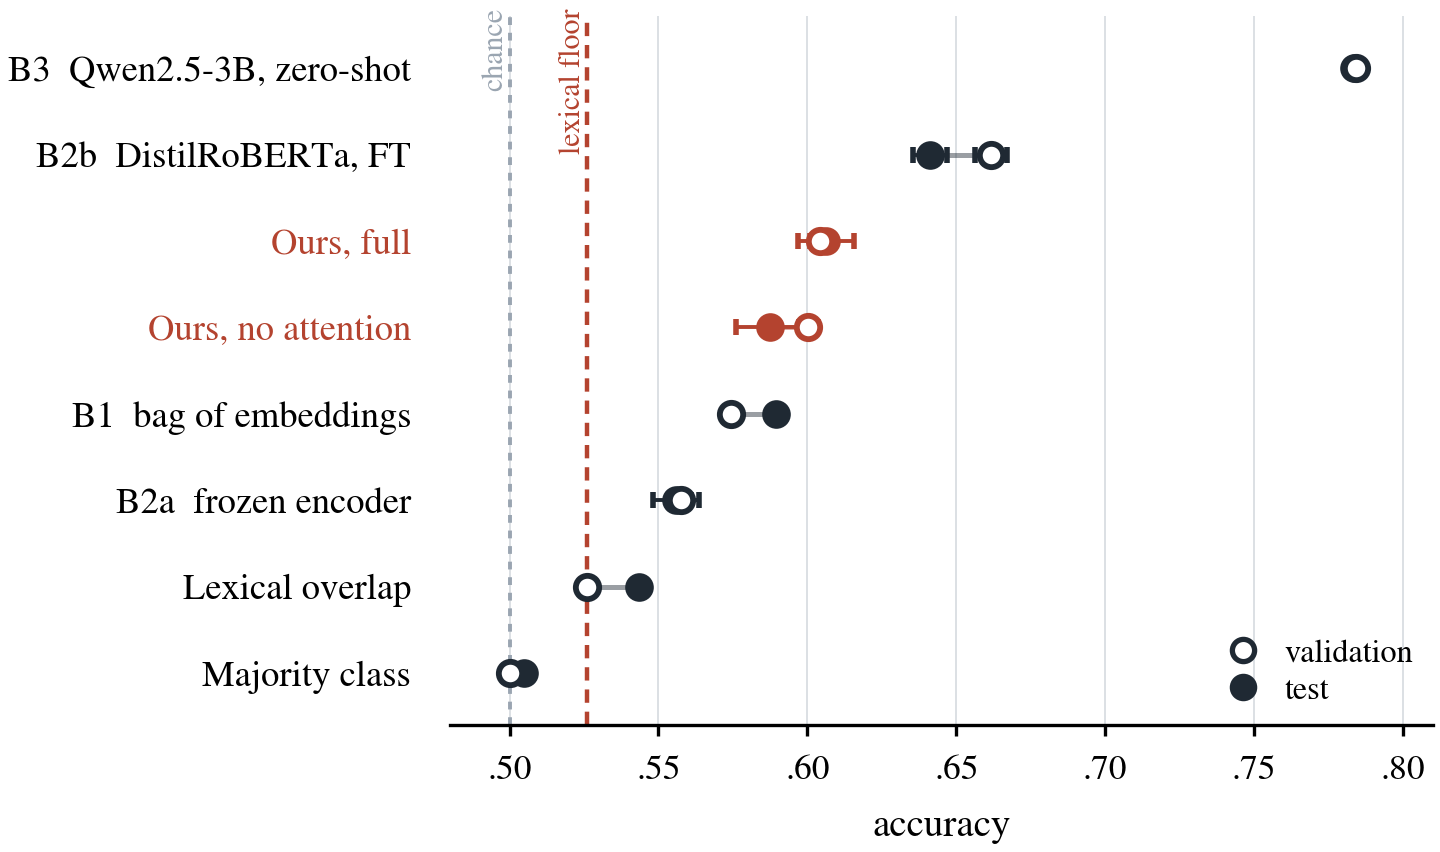
\includegraphics[width=0.80\columnwidth]{fig5_baselines.png}
  \caption{Validation (hollow) and test (filled) accuracy per system. Dashed
  lines mark the majority baseline and the lexical floor; axis truncated.}
  \label{fig:base}
\end{figure}

\paragraph{B0, the lexical floor}
A heuristic selecting whichever candidate shares more words with the goal
reaches $0.5259$ on validation, the floor a learned model must clear.

\paragraph{B1, bag of embeddings}
B1 isolates the sequence model: the base configuration with the bidirectional
LSTM replaced by a masked mean over word embeddings (Section~\ref{sec:scoring}
without $d_k$).

\paragraph{B2a, frozen pretrained encoder}
We freeze all 82M encoder parameters of \texttt{distilroberta-base}
\citep{sanh2019distilbert,liu2019roberta} and train only the final classifier
($769$ parameters) on the frozen \texttt{[CLS]} output of each $(g,s_k)$
pair, which reduces to logistic regression on fixed features. B2a lands
$3.17$ points above the floor but $4.27$ below our base ($|t| = 12.8$).

\paragraph{B2b, fine-tuned pretrained encoder}
B2b differs in one variable, the encoder being unfrozen, with pairs truncated
to $128$ subword tokens through \texttt{AutoModelForMultipleChoice} and AdamW
at $2 \times 10^{-5}$ \citep{mosbach2021stability}. Because the pair is
controlled, the $10.41$ point step measures what adapting a pretrained
representation is worth: almost all of it is released by fine-tuning, not
carried by the frozen features.

\paragraph{B3, Qwen2.5-3B zero-shot}
B3 estimates the headroom from pretraining at 3B parameters with no task
adaptation: each candidate scored under \texttt{Qwen/Qwen2.5-3B-Instruct} by
the mean log-likelihood of its tokens under the prompt
\texttt{Goal: \{g\}\textbackslash nSolution: \{s\_k\}}
\citep{bisk2020piqa}, one deterministic fp16 run. The pretraining corpus very
likely contains PIQA-style questions, so the gap measures pretraining rather
than architecture.

\subsection{Evaluation metrics}
\label{sec:metrics}

We evaluate with accuracy, the proportion of instances for which the argmax
of $f$ coincides with the gold label. The task is a forced choice with
balanced labels, and the only two errors --- choosing $s_1$ when $s_2$ is
correct, and the reverse --- are symmetric, with neither candidate privileged
as a positive class. Accuracy is therefore the natural measure and the one
used in the original PIQA work \citep{bisk2020piqa}.

\section{Results and Analysis}
\label{sec:results}

\subsection{Ablation studies}
\label{sec:ablation}

Each block of Table~\ref{tab:ablation} answers one question. The first asks
whether any mechanism helps alone: A1 should weight informative solution
tokens, A2 informative goal tokens, A3 the differences between near-duplicate
candidates. The second asks why A1 underperforms, adding one refinement at a
time --- mean mixing (does keeping the mean help?), fixed $\sqrt{D}$ scaling
(is the softmax saturating?), learned $T$ (can it beat $\sqrt{D}$?), and the
full-goal residual (does token-level conditioning beat one pooled query?).
The third asks whether A2 or A3 still contributes once the rest is present.
All runs share the split, backbone, scorer, optimiser, budget and seeds
$0,1,2$; except for the component under test, settings stay fixed, and no
attention is the reference.

\begin{table}[tb]
  \centering\small
  \begin{tabular}{@{}lcc@{}}
    \toprule
    \textbf{Configuration} & \textbf{Validation} & \textbf{$\Delta$}\\
    \midrule
    No attention (reference) & $0.6003 \pm 0.0032$ & $0.0000$\\
    A1 (learned-query)       & $0.5901 \pm 0.0034$ & $-0.0102$\\
    A2 only                  & $0.5919 \pm 0.0029$ & $-0.0084$\\
    A3 only                  & $0.5999 \pm 0.0053$ & $-0.0004$\\
    A2 + A3                  & $0.6042 \pm 0.0069$ & $+0.0039$\\
    \midrule
    A1 + mean mix            & $0.5870 \pm 0.0046$ & $-0.0133$\\
    \;\;+ fixed $\sqrt{D}$ scaling & $0.5938 \pm 0.0011$ & $-0.0065$\\
    \;\;+ learned temperature      & $0.5959 \pm 0.0025$ & $-0.0044$\\
    Final A1                 & $0.5963 \pm 0.0034$ & $-0.0040$\\
    \midrule
    Full $-$ A2              & $0.5999 \pm 0.0030$ & $-0.0004$\\
    Full $-$ A3              & $0.5918 \pm 0.0054$ & $-0.0085$\\
    Full model               & $0.6042 \pm 0.0032$ & $+0.0039$\\
    \bottomrule
  \end{tabular}
  \caption{Validation ablations against the no-attention reference, mean
  $\pm$ sd over seeds $0,1,2$. Final A1 $=$ mean mix $+$ learned $T$ $+$
  full-goal residual; Full $=$ that plus A2 and A3.}
  \label{tab:ablation}
\end{table}

In Table~\ref{tab:ablation}, only learned-query A1 and unscaled A1 with mean
mixing cross the $0.0099$ threshold, and both are worse; the full model and
A2$+$A3 share the highest mean but gain only $0.0039$, so no separable
attention effect appears.

The staged A1 rows show scaling recovering much of the loss from unscaled
mean mixing --- about $0.0069$ fixed and $0.0090$ learned in seed-paired
comparisons --- but never exceeding no attention. Because the first A1 row is
a learned-query control while later variants use a goal-conditioned query,
their difference cannot be attributed to mixing alone. The fixed-scaling
comparison follows \citet{vaswani2017attention}, the learned variant
\citet{dufter2020temperature}, and the full-goal residual query-aware token
representations \citep{seo2017bidaf} with a zero-initialised ReZero gate
\citep{bachlechner2021rezero}.

Leave-one-out answers the third question negatively (Figure~\ref{fig:abl}):
removing A2 costs $0.0043$ and A3 $0.0124$, but Full~$-$~A3 still sits within
$0.0099$ of the reference, so neither earns a separable place.

\begin{figure}[tb]
  \centering
  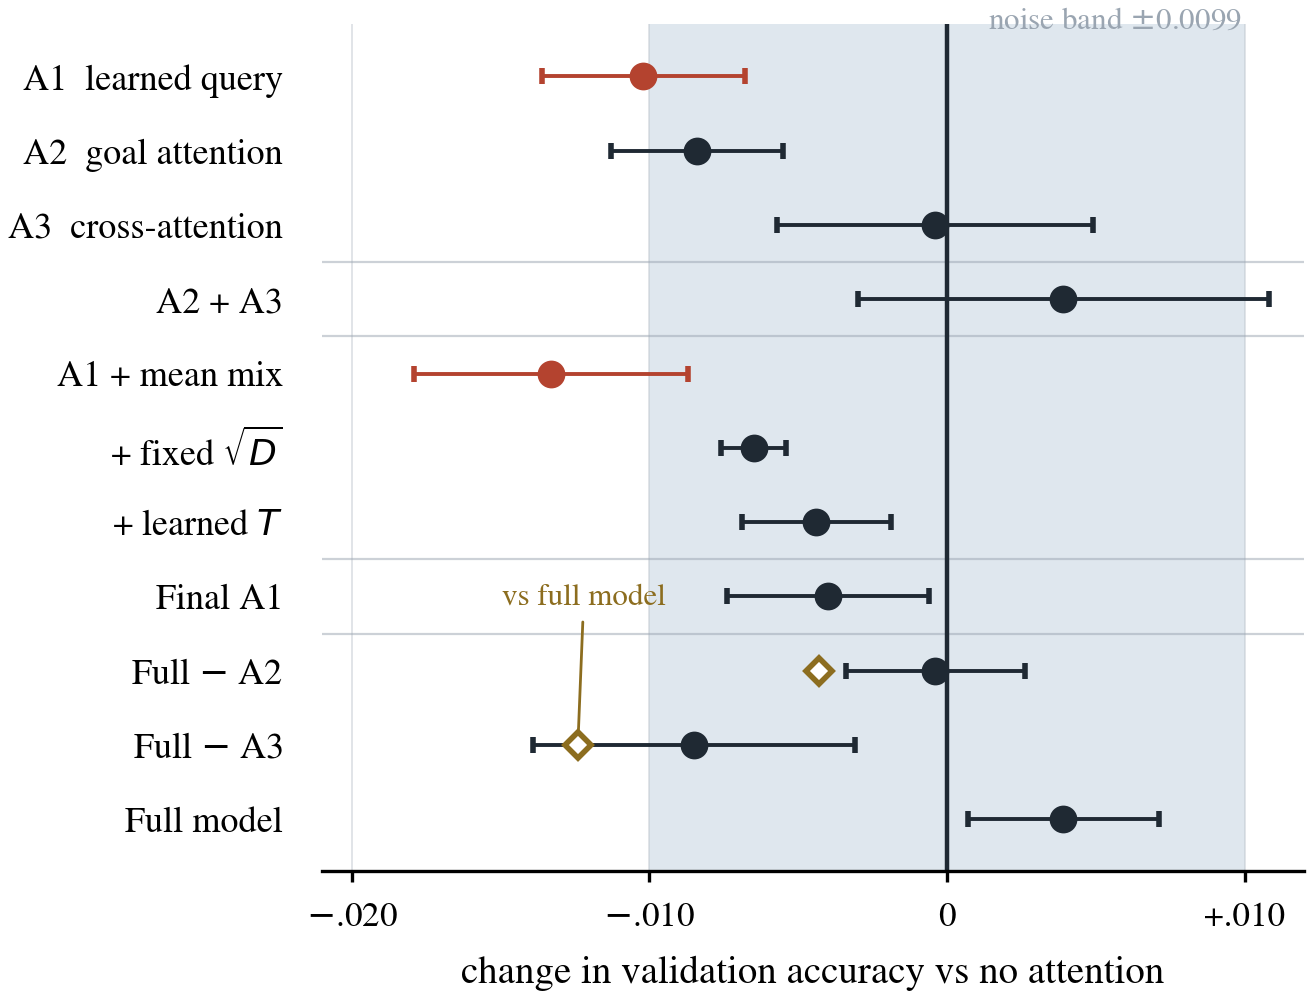
\includegraphics[width=0.80\columnwidth]{fig6_ablation.png}
  \caption{Attention ablations against the no-attention reference. The band
  spans the $0.0099$ threshold; the two red points are the only
  configurations outside it, both negative. Open diamonds give the
  leave-one-out difference from the full model.}
  \label{fig:abl}
\end{figure}

\subsection{Qualitative analysis of attention}
\label{sec:qual}

The temperature settings first show what A1 attends to
(Figure~\ref{fig:temp}). On validation row $0$ --- remove sprouts from
potatoes, gold answer the vegetable peeler --- all three A1 checkpoints
predict correctly, but over 23 real tokens, against a uniform $0.043$, the
scaled variants peak at only $0.056$ and $0.063$. The unscaled one reaches
$0.126$ yet weights shared words above the deciding contrast, so scaling makes
A1 behave like mean pooling.


\begin{figure}[tb]
  \centering
  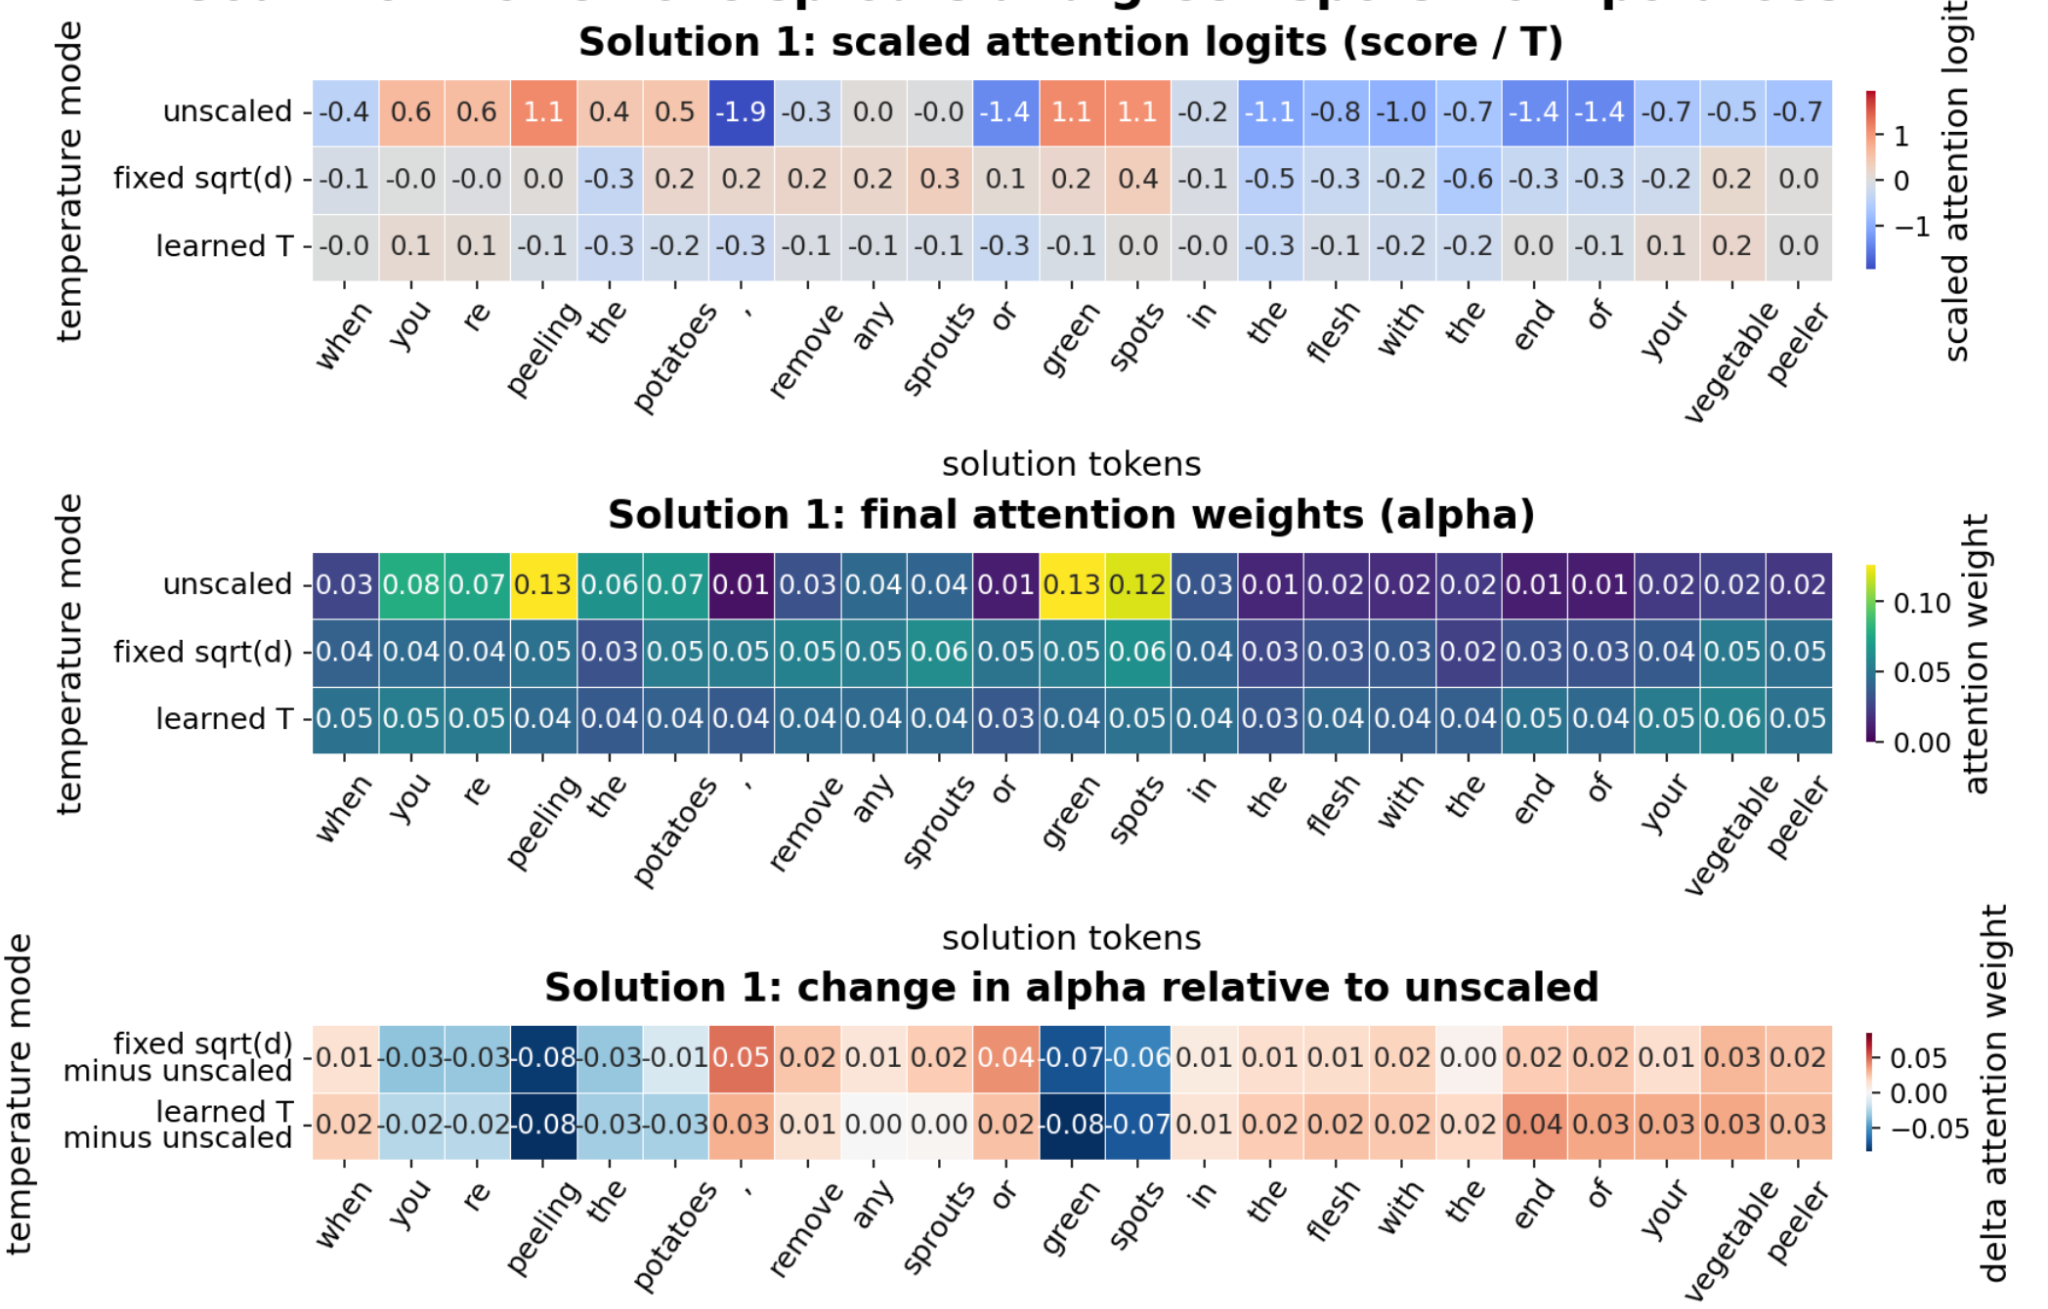
\includegraphics[width=0.88\columnwidth]{fig7a_temp_sol1.png}
  \caption{A1 under three temperature settings, validation row $0$,
  solution~1: scaled logits, weights $\alpha$, and the change in $\alpha$
  against the unscaled checkpoint.}
  \label{fig:temp}
\end{figure}

Figures~\ref{fig:heat1} and~\ref{fig:heat3} compare a success and a failure
on row $635$, goal \textit{Loosen stuck drawers}: solution~1 rubs bar soap on
the handles, solution~2 on the runners. The gold answer is solution~2, taken
by the full model with $P = 0.617$ while the A1 $+$ mean mix ablation takes
the wrong one at $P = 0.938$.

\begin{figure}[tb]
  \centering
  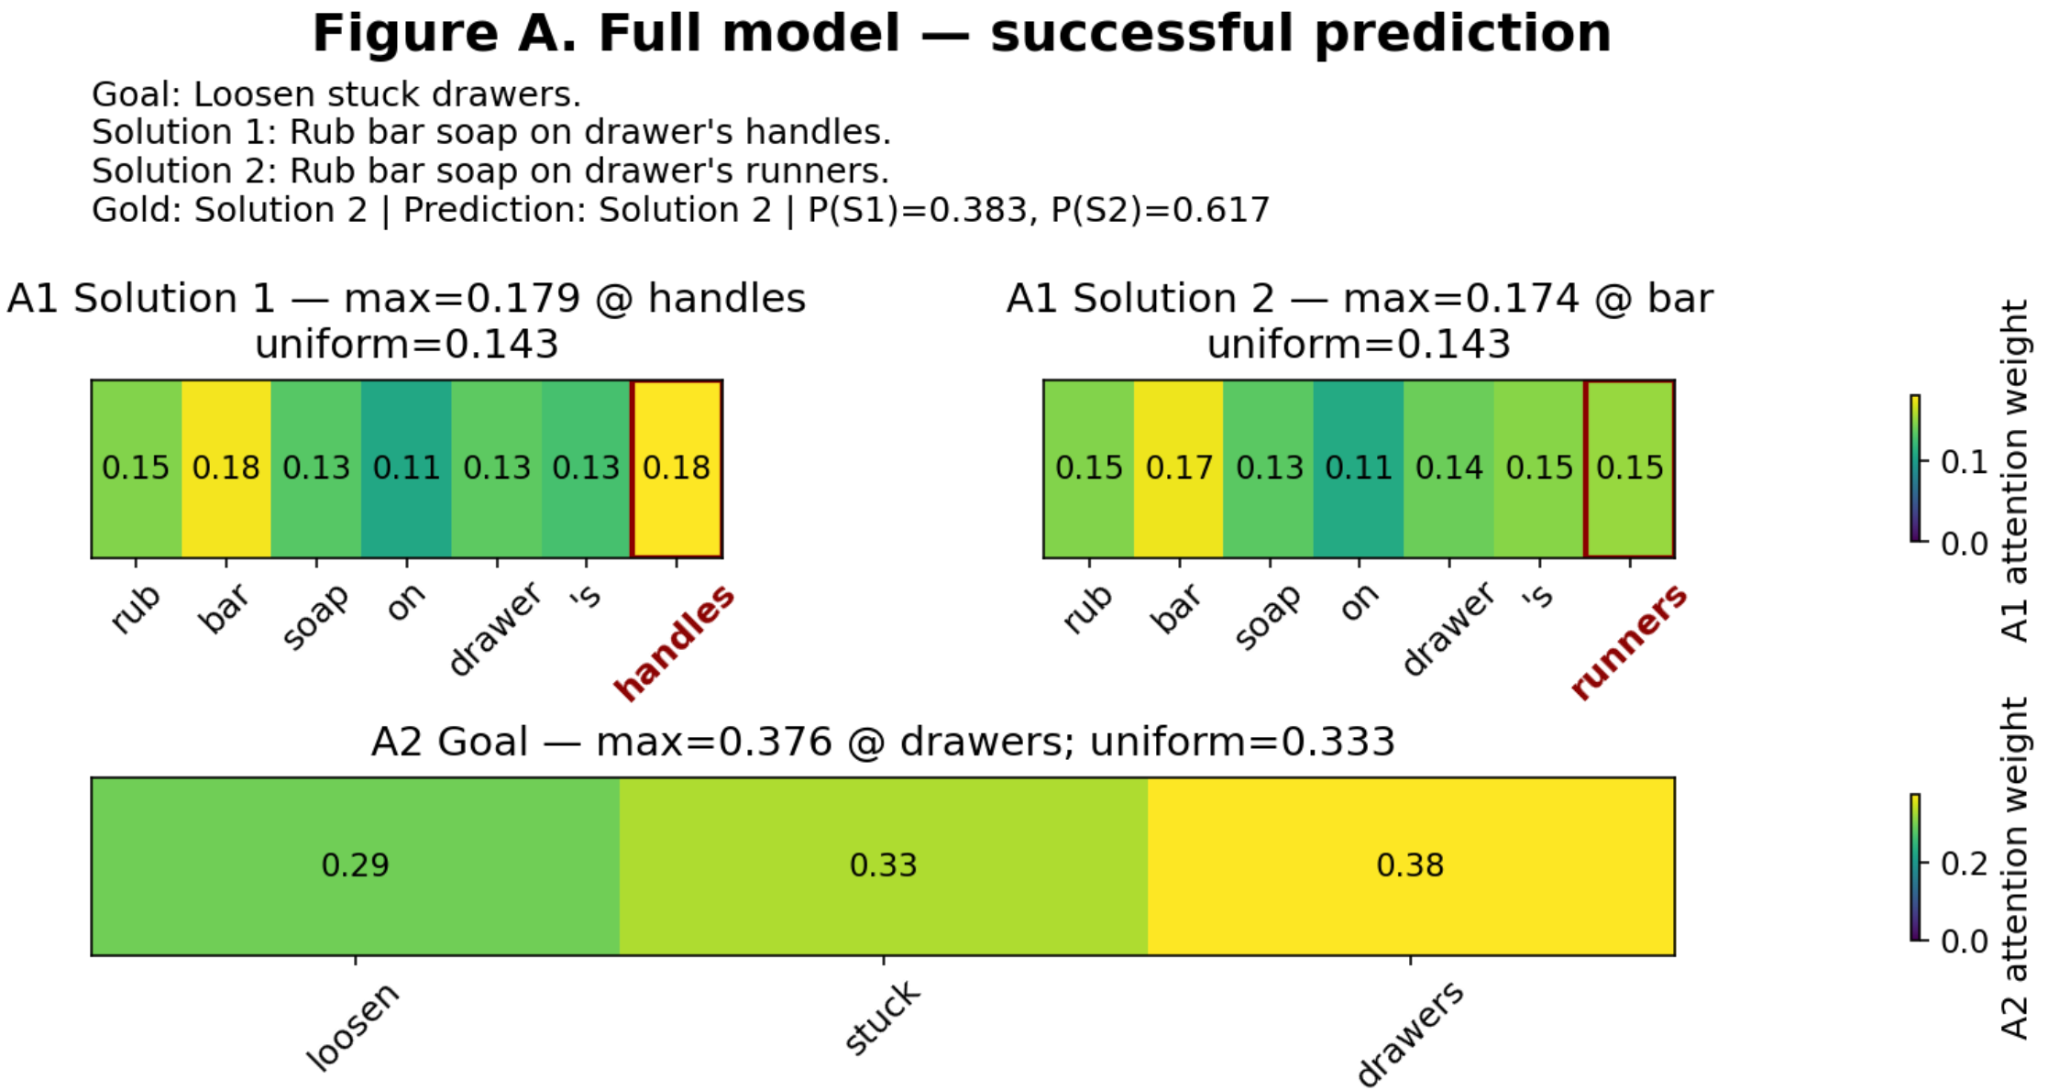
\includegraphics[width=0.88\columnwidth]{fig8a_full_a1a2.png}\\[1pt]
  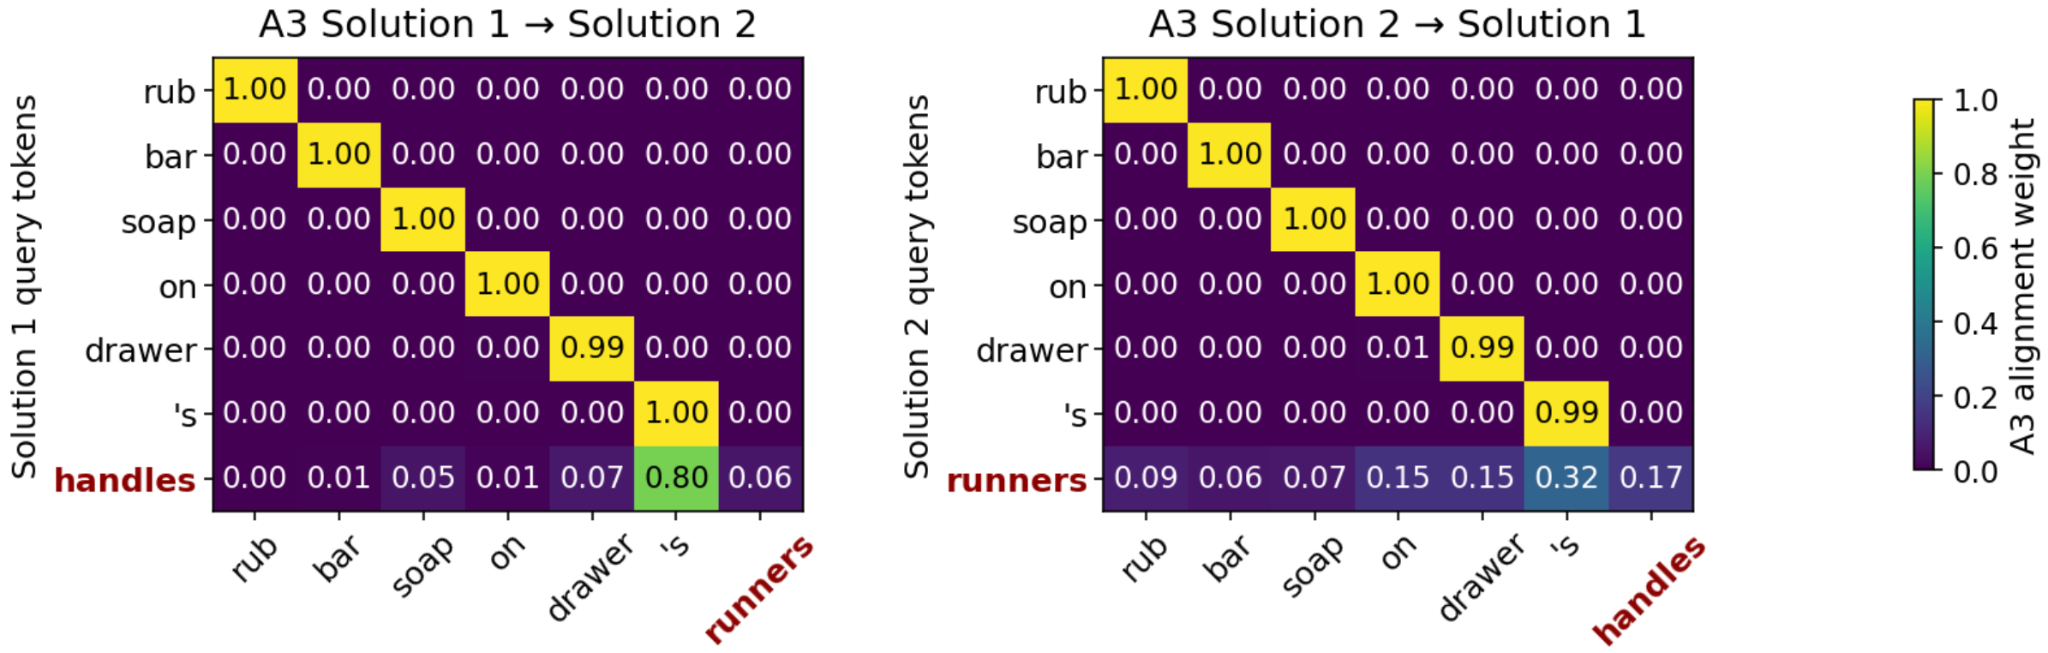
\includegraphics[width=0.88\columnwidth]{fig8b_full_a3.png}
  \caption{Full model, correct prediction, validation row $635$. Top: A1 and
  A2 attention. Bottom: A3 cross-solution alignment; red labels mark tokens
  outside shared blocks.}
  \label{fig:heat1}
\end{figure}

In the success both A1 distributions are flat, peaking at $0.179$ and $0.174$
against a seven-token uniform of $0.143$, so A1 does not mark
\textit{runners} as decisive, and A2 is equally diffuse.

A3 is the one component with visible structure: the six shared tokens align
almost one to one at $0.99$ to $1.00$, separating the shared frame from the
two distinguishing nouns --- which do not align with each other, so A3 shows
where the candidates differ without settling which wins.

\begin{figure}[tb]
  \centering
  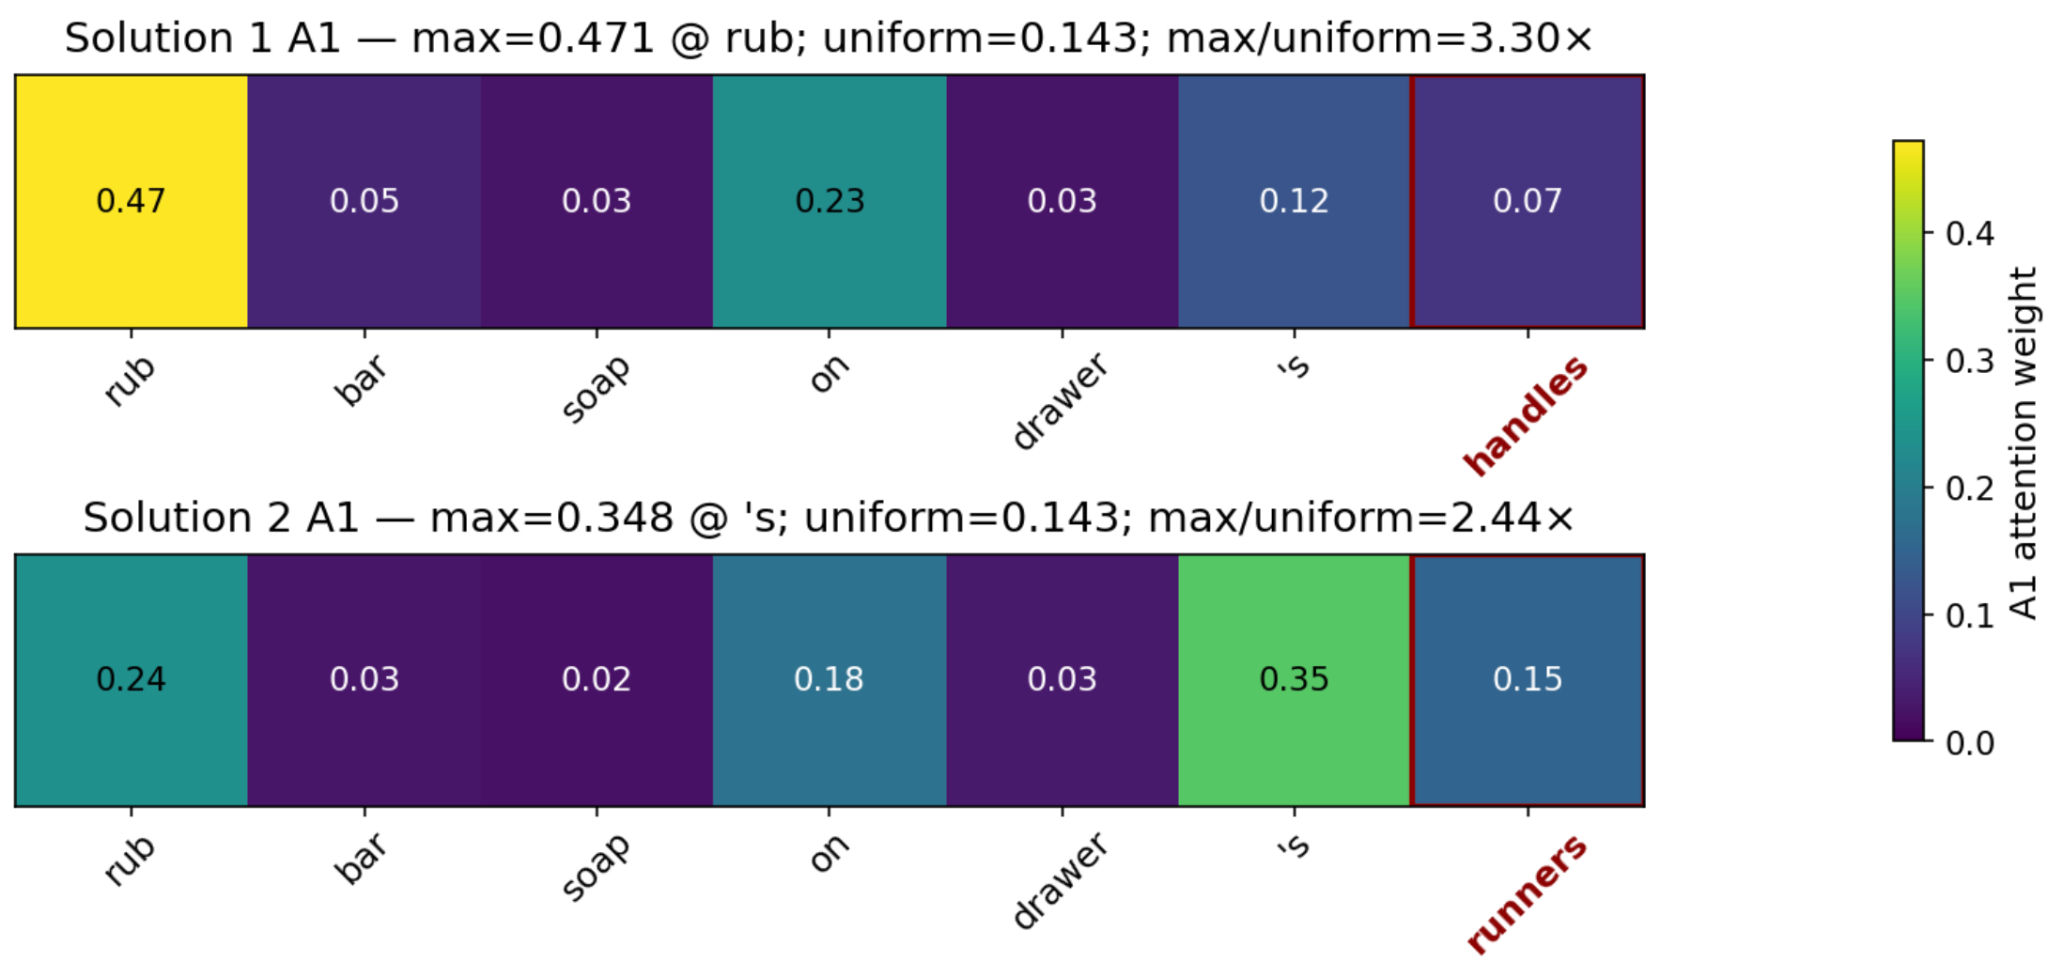
\includegraphics[width=0.88\columnwidth]{fig8c_ablation_err.png}
  \caption{A1 attention for the A1 $+$ mean mix ablation's highest-confidence
  error, row $635$. This configuration has neither A2 nor A3.}
  \label{fig:heat3}
\end{figure}

The failed ablation concentrates sharply in unhelpful places: $0.471$ on the
shared verb \textit{rub}, $3.30$ times uniform, while \textit{handles} and
\textit{runners} get $0.071$ and $0.151$; its mixing weight of $0.810$ lets
that misplaced concentration dominate the masked mean. Attention sharpness is
therefore not a reliable proxy for correct reasoning. Being different
checkpoints, the two describe behaviour rather than isolate one component.

\subsection{Overall performance comparison}
\label{sec:overall}

\begin{table}[tb]
  \centering\small
  \setlength{\tabcolsep}{2.5pt}
  \begin{tabular}{@{}lcc@{}}
    \toprule
    \textbf{System} & \textbf{Validation} & \textbf{Test}\\
    \midrule
    Majority class & $0.5002$ & $0.5049$\\
    Lexical overlap & $0.5259$ & $0.5435$\\
    \midrule
    B1 \ bag of embeddings & $0.5745 \pm 0.0023$ & $0.5896 \pm 0.0019$\\
    B2a \ frozen encoder & $0.5576 \pm 0.0034$ & $0.5559 \pm 0.0077$\\
    \midrule
    \rowcolor{ourrow}
    \textbf{Ours, no attention} & $0.6003 \pm 0.0032$ & $0.5874 \pm 0.0094$\\
    \rowcolor{ourrow}
    \textbf{Ours, full} & $0.6042 \pm 0.0032$ & $\mathbf{0.6063 \pm 0.0094}$\\
    \midrule
    B2b \ DistilRoBERTa, FT & $0.6617 \pm 0.0054$ & $0.6411 \pm 0.0057$\\
    B3 \ Qwen2.5-3B, 0-shot & $0.7844$ & $0.7835$\\
    \bottomrule
  \end{tabular}
  \caption{Accuracy on both splits, grouped by family. Learned systems use
  seeds $0,1,2$, both columns from one execution. Separability threshold
  $0.0099$ on validation, $0.0187$ on test.}
  \label{tab:overall}
\end{table}

Table~\ref{tab:overall} reports both splits. Four observations follow.

\textbf{(1)} Every step of the validation hierarchy clears the seed-noise
threshold under Welch's test except our own attention stack, where the
$0.0039$ between the full model and the backbone sits well inside it
($|t| = 1.21$).

\textbf{(2)} Frozen, the pretrained checkpoint scores $4.27$ points
\emph{below} our $1.5$M-parameter model; unfrozen, $6.14$ above. That $10.41$
point step exceeds every architectural difference we measured, and zero-shot
Qwen2.5-3B dwarfs both at $18.02$ above us.

\textbf{(3)} The test column preserves the ordering with one exception, ours:
B1 rises while our no-attention model falls, so the $2.58$ point validation
gap does not survive the held-out split. Our two configurations also carry the
largest test spreads, $0.0094$ --- three times their validation spread.

\textbf{(4)} The full attention stack is nonetheless the only system that does
not lose ground on test, $0.0189$ above the backbone against a comparable
threshold of $0.0187$. Both reproduce exactly under the controls of
Section~\ref{sec:training}, so the comparison can be paired: the full model
wins on all three seeds, at a paired $t$ of $2.57$ against our cutoff of
$4.3$. We do not claim attention helps, only that this configuration held its
ground on every seed --- a direction three seeds cannot separate from a
favourable draw.

\section{Conclusion}
\label{sec:conclusion}

Our model clears the lexical floor by a wide margin, but eight backbone
hyperparameters and every attention configuration sit inside the seed-noise
band. The weights show why: scaling flattens the attention, the flattened
version performs better, and a flat distribution is mean pooling by another
name --- the mechanism is reporting that no small set of positions is
decisive. What separates the stronger baselines from ours is how much text
they have seen, not how they are wired: the signal in PIQA is world knowledge,
and $13{,}696$ instances do not hold enough of it. The methodological lesson
is the one we did not start with --- measuring the noise floor before reading
any difference. Without it we would have reported the $0.0039$ gain as a
result.

\paragraph{Limitations and future work}
The embedding matrix holds $75.5\%$ of the parameters and is trained from
scratch, so the ceiling is bounded by the training set as much as the
architecture; the Transformer was set aside on data scale, not by experiment;
the cross-attention is quadratic in candidate length; and three seeds resolve
only $0.0112$. A larger pretrained encoder and more seeds follow.

\clearpage
\section*{Team Contributions}

Daniel designed and implemented the main model, ran the hyperparameter sweep,
the convergence study and the seed-noise protocol, wrote Section~\ref{sec:method}
and Sections~\ref{sec:data}--\ref{sec:hparams} and~\ref{sec:metrics}, and
integrated and submitted the report. Ray implemented the attention mechanisms
and their refinements, ran the ablations, produced the attention
visualisations, and wrote Section~\ref{sec:refine} and
Sections~\ref{sec:ablation} and~\ref{sec:qual}. Vika implemented and ran the
four baseline families, and wrote Section~\ref{sec:intro},
Section~\ref{sec:baselines}, Section~\ref{sec:overall} and
Section~\ref{sec:conclusion}. All three authors reviewed the final manuscript.

\bibliography{references}

\end{document}
